%%
%% This is file `sample-authordraft.tex',
%% generated with the docstrip utility.
%%
%% The original source files were:
%%
%% samples.dtx  (with options: `authordraft')
%% 
%% IMPORTANT NOTICE:
%% 
%% For the copyright see the source file.
%% 
%% Any modified versions of this file must be renamed
%% with new filenames distinct from sample-authordraft.tex.
%% 
%% For distribution of the original source see the terms
%% for copying and modification in the file samples.dtx.
%% 
%% This generated file may be distributed as long as the
%% original source files, as listed above, are part of the
%% same distribution. (The sources need not necessarily be
%% in the same archive or directory.)
%%
%% The first command in your LaTeX source must be the \documentclass command.
\documentclass[sigconf,authordraft]{acmart}

%%
%% \BibTeX command to typeset BibTeX logo in the docs
\AtBeginDocument{%
  \providecommand\BibTeX{{%
    \normalfont B\kern-0.5em{\scshape i\kern-0.25em b}\kern-0.8em\TeX}}}

%% Rights management information.  This information is sent to you
%% when you complete the rights form.  These commands have SAMPLE
%% values in them; it is your responsibility as an author to replace
%% the commands and values with those provided to you when you
%% complete the rights form.
\setcopyright{acmcopyright}
\copyrightyear{2020}
\acmYear{2020}
% \acmDOI{10.1145/1122445.1122456}

%% These commands are for a PROCEEDINGS abstract or paper.
\acmConference[CIKM '20]{29th ACM International Conference on Information and Knowledge Management}{October 19--23, 2020}{ONLINE}
\acmBooktitle{CIKM '20: ACM International Conference on Information and Knowledge Management,
  October 19--23, 2020, ONLINE}
% \acmPrice{15.00}
% \acmISBN{978-1-4503-XXXX-X/18/06}


%%
%% Submission ID.
%% Use this when submitting an article to a sponsored event. You'll
%% receive a unique submission ID from the organizers
%% of the event, and this ID should be used as the parameter to this command.
%%\acmSubmissionID{123-A56-BU3}

%%
%% The majority of ACM publications use numbered citations and
%% references.  The command \citestyle{authoryear} switches to the
%% "author year" style.
%%
%% If you are preparing content for an event
%% sponsored by ACM SIGGRAPH, you must use the "author year" style of
%% citations and references.
%% Uncommenting
%% the next command will enable that style.
%%\citestyle{acmauthoryear}

%\newcommand{\defeq}{\stackrel{\mathclap{\normalfont\mbox{def}}}{=}}
\newcommand{\R}{\mathbb{R}}
\newcommand{\w}{\pmb{w}}
\newcommand{\al}{\pmb{\alpha}}


%%
%% end of the preamble, start of the body of the document source.
\begin{document}

%%
%% The "title" command has an optional parameter,
%% allowing the author to define a "short title" to be used in page headers.
\title{Feature and Instance Selection via Strong Rule}

%%
%% The "author" command and its associated commands are used to define
%% the authors and their affiliations.
%% Of note is the shared affiliation of the first two authors, and the
%% "authornote" and "authornotemark" commands
%% used to denote shared contribution to the research.
%%%% author starts here
% \author{Ben Trovato}
% \authornote{Both authors contributed equally to this research.}
% \email{trovato@corporation.com}
% \orcid{1234-5678-9012}
% \author{G.K.M. Tobin}
% \authornotemark[1]
% \email{webmaster@marysville-ohio.com}
% \affiliation{%
%   \institution{Institute for Clarity in Documentation}
%   \streetaddress{P.O. Box 1212}
%   \city{Dublin}
%   \state{Ohio}
%   \postcode{43017-6221}
% }

% \author{Lars Th{\o}rv{\"a}ld}
% \affiliation{%
%   \institution{The Th{\o}rv{\"a}ld Group}
%   \streetaddress{1 Th{\o}rv{\"a}ld Circle}
%   \city{Hekla}
%   \country{Iceland}}
% \email{larst@affiliation.org}

% \author{Valerie B\'eranger}
% \affiliation{%
%   \institution{Inria Paris-Rocquencourt}
%   \city{Rocquencourt}
%   \country{France}
% }

% \author{Aparna Patel}
% \affiliation{%
%  \institution{Rajiv Gandhi University}
%  \streetaddress{Rono-Hills}
%  \city{Doimukh}
%  \state{Arunachal Pradesh}
%  \country{India}}

% \author{Huifen Chan}
% \affiliation{%
%   \institution{Tsinghua University}
%   \streetaddress{30 Shuangqing Rd}
%   \city{Haidian Qu}
%   \state{Beijing Shi}
%   \country{China}}

% \author{Charles Palmer}
% \affiliation{%
%   \institution{Palmer Research Laboratories}
%   \streetaddress{8600 Datapoint Drive}
%   \city{San Antonio}
%   \state{Texas}
%   \postcode{78229}}
% \email{cpalmer@prl.com}

% \author{John Smith}
% \affiliation{\institution{The Th{\o}rv{\"a}ld Group}}
% \email{jsmith@affiliation.org}

% \author{Julius P. Kumquat}
% \affiliation{\institution{The Kumquat Consortium}}
% \email{jpkumquat@consortium.net}

%%
%% By default, the full list of authors will be used in the page
%% headers. Often, this list is too long, and will overlap
%% other information printed in the page headers. This command allows
%% the author to define a more concise list
%% of authors' names for this purpose.
% \renewcommand{\shortauthors}{Trovato and Tobin, et al.}

%%
%% The abstract is a short summary of the work to be presented in the
%% article.
\begin{abstract}
\end{abstract}
%%
%% The code below is generated by the tool at http://dl.acm.org/ccs.cfm.
%% Please copy and paste the code instead of the example below.
%%
\begin{CCSXML}
<ccs2012>
 <concept>
  <concept_id>10010520.10010553.10010562</concept_id>
  <concept_desc>Computer systems organization~Embedded systems</concept_desc>
  <concept_significance>500</concept_significance>
 </concept>
 <concept>
  <concept_id>10010520.10010575.10010755</concept_id>
  <concept_desc>Computer systems organization~Redundancy</concept_desc>
  <concept_significance>300</concept_significance>
 </concept>
 <concept>
  <concept_id>10010520.10010553.10010554</concept_id>
  <concept_desc>Computer systems organization~Robotics</concept_desc>
  <concept_significance>100</concept_significance>
 </concept>
 <concept>
  <concept_id>10003033.10003083.10003095</concept_id>
  <concept_desc>Networks~Network reliability</concept_desc>
  <concept_significance>100</concept_significance>
 </concept>
</ccs2012>
\end{CCSXML}

% \ccsdesc[500]{Computer systems organization~Embedded systems}
% \ccsdesc[300]{Computer systems organization~Redundancy}
% \ccsdesc{Computer systems organization~Robotics}
% \ccsdesc[100]{Networks~Network reliability}

%%
%% Keywords. The author(s) should pick words that accurately describe
%% the work being presented. Separate the keywords with commas.
\keywords{classification, large scale, feature selection, instance selection}

%% A "teaser" image appears between the author and affiliation
%% information and the body of the document, and typically spans the
%% page.
% \begin{teaserfigure}
%   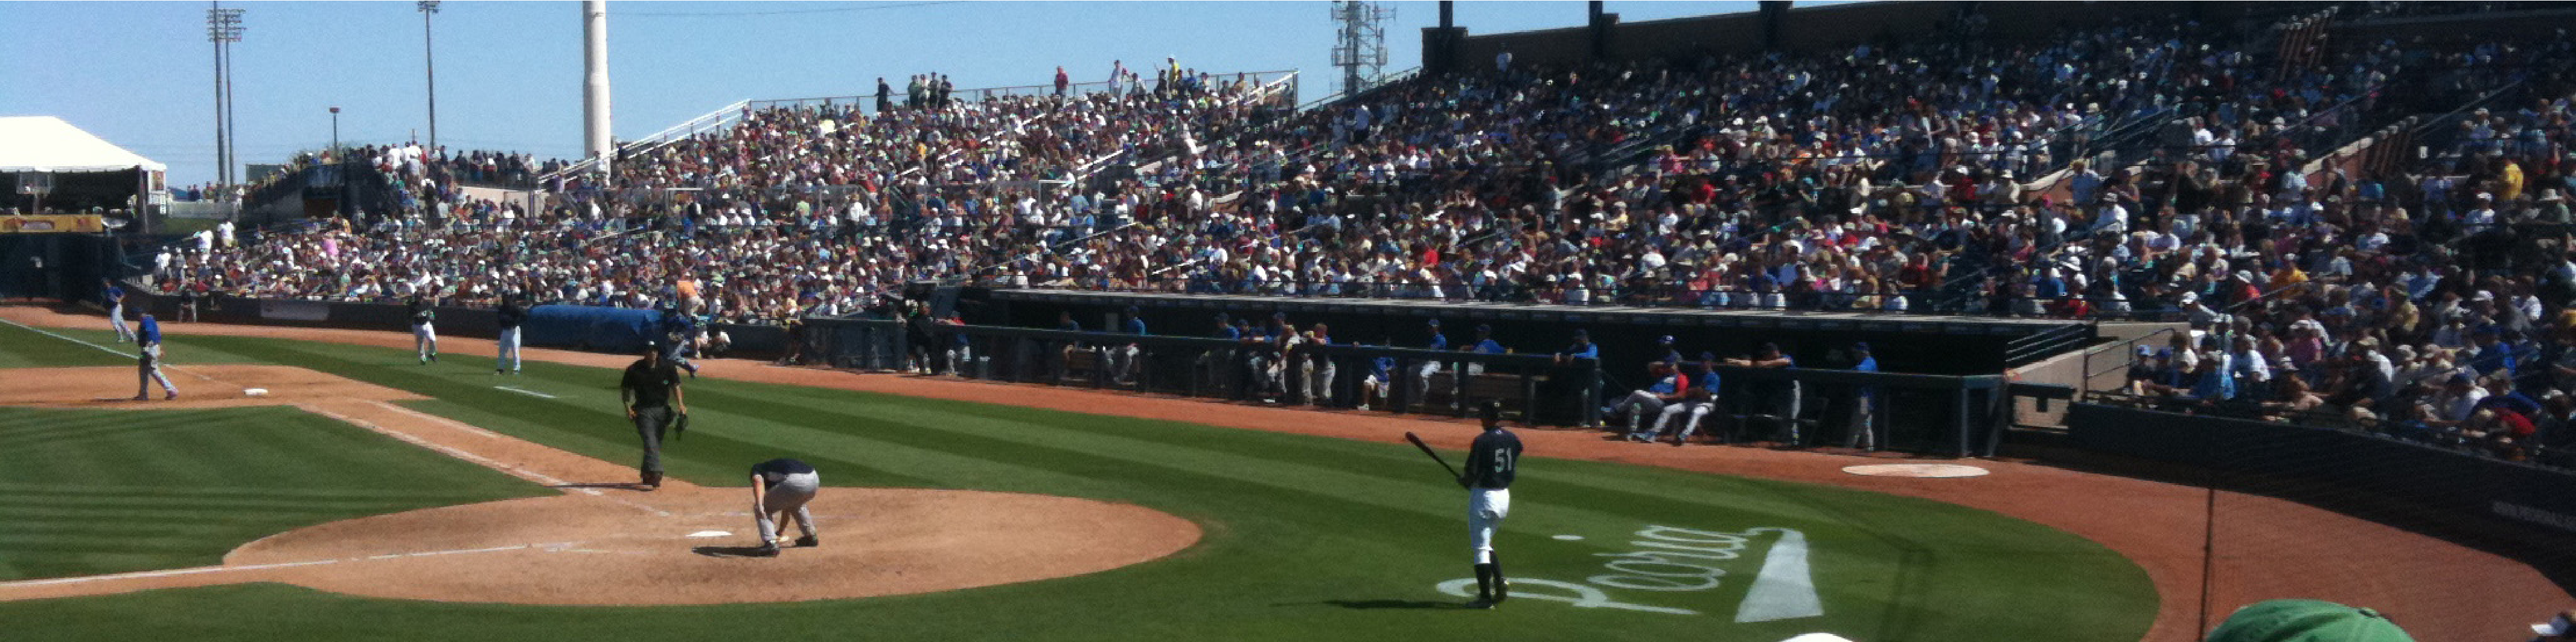
\includegraphics[width=\textwidth]{sampleteaser}
%   \caption{Seattle Mariners at Spring Training, 2010.}
%   \Description{Enjoying the baseball game from the third-base
%   seats. Ichiro Suzuki preparing to bat.}
%   \label{fig:teaser}
% \end{teaserfigure}

%%
%% This command processes the author and affiliation and title
%% information and builds the first part of the formatted document.
\maketitle

\section{Introduction}

\section{Related Work}

\section{Method}
\subsection{Feature Selection}
Strong rules have been used for discarding less important features in a lasso related regression or classification problems\cite{tibshirani2012strong,ghaoui2010safe}. In \cite{tibshirani2012strong}, authors considered strong rule for binary logistic regression problem ($y \in \{0, 1\}$, $\pmb{x} \in \R^{d}$, wherein $d$ is the feature dimension):

\begin{align}
    p(y=1 | \pmb{x}; \w) = \frac{1}{1 + \exp(-\pmb{x}^T\w)}
\end{align}

For simplicity purposes, we write $p_i = p(y_i | x_i; \pmb{w})$. Based on Regularized Empirical Risk Minimization, we are seeking an optimal solution of $\hat{\pmb{w}}$ that minimizes the negative log-likelihood on the given training dataset $D=  \{\pmb{y}, \pmb{X}\} = \{(y_i, \pmb{x}_i)\}_{i=1}^{n}$ with $n$ as the number of data,

\begin{align}
    &\hat{\w} = \arg \min_{\w\in \R^{d}} \sum_{i=1}^n {\phi_i(\pmb{x}_i^T\pmb{w}) + \lambda g(\pmb{w})} \text{ wherein} \label{eq:loss} \\
    &\phi(\pmb{x}_i^T\w) = y_i \log p_i + (1-y_i) \log (1-p_i) \text{ and } \\
    &g(\w) = ||\w||_1
    % \hat{\w} &= \arg\min_{\w\in \R^{d}} - \sum_{i=1}^n \left( y_i \log p_i + (1-y_i) \log (1-p_i) \right) + \lambda ||\w||_1  
\end{align}

$\lambda$ is a hyper-parameter for the lasso penalty. With a large value of $\lambda$, the optimal solution $\w$ may yield to a sparse vector, especially when the number of features $d$ is large. Now suppose the sparse solution is given in advance: a subset of non-zero predictors $S \in \{1,2,\dots,n\}$ and the complement of $S$ set is $S'$, which has $\hat{\w}_{j: j \in S} \neq 0$ and $\hat{\w}_{j: j \in S'} = 0$. In this case, we could first discard the features in $S'$, and then apply an optimization method to solve (\ref{eq:loss}) using features in $S$ only. The feature selection may not just reduce computational time and memory, especially for coordinated descent based optimizer \cite{friedman2010regularization}, but also prevents the over-fitting. 

In \cite{tibshirani2012strong}, authors proposed a general \textit{strong rule} for discarding features in the lasso-type loss function. For the binary logistic regression, we define a score $s_j$ for discarding the $j$-th feature via the \textit{strong rule}:

\begin{align}
    s_j = |\pmb{x}_j^T (\pmb{y} - \pmb{\bar{p}})| < \epsilon
    \label{eq:strongrule}
\end{align}

where $\pmb{x}_j$ is the $j$-th feature column, $\pmb{\bar{p}} = \pmb{1} \frac{\sum_{i=1}^n y_i}{n}$ is a vector of the prior probability of positive instances, and a non-negative $\epsilon$ is a threshold for filtering out features and it is related to the strength of lasso penalty $\lambda$. From (\ref{eq:strongrule}), the strong rule produces the priority scores for all features by looking at the inner product of each feature with the residuals. Given that $\bar{\pmb{p}} \in (0,1)$, it is not hard to notice that residuals for positive instance are always positive, and are always negative for negative instances. Furthermore, if assuming that the features are positive, binary and scaled to unit length ($\sum_{i=1}^{n} \pmb{x}_{ij} = 1 $ for all $j$, and any two non-zero feature values in $j$-th column equal to each other), it can be verified that \textit{unique features}, who appear either only in positive instances or only in negative instances, have larger priority scores than the features appearing in both positive and negative instances under some assumption (see Appendix \ref{appendix:feature_selection}). The lowest priority will happen to a feature that is distributed evenly in positive and negative instances (\textit{common feature}), e.g. stop words in a text classification problem. 

The strong rule can be easily applied to remove inactive features, i.e. more common features, but it may mistakenly discard some active features. To reduce the chances of making mistakes, one way is to keep a larger portion of features in the model to prevent discarding more active features, or to combine with KKT (Karush-Kuhn-Tucker) conditions to ensure that there is no active feature being discarded\cite{tibshirani2012strong}. In this paper, we will address this erroneous issue by an unaggressive strong rule: using a larger threshold $\epsilon$ to save a larger portion of features in the model for training. 

In practice, many optimizers, especially for coordinate coordinate descent and ascent methods\cite{friedman2010regularization}, take full advantage of feature selection, to reduce the computational cost in training time and memory. On the other hand, feature selection may also prevent over-fitting by limiting the model complexity\cite{reunanen2003overfitting}. 

\subsection{Instance Selection}

In addition to a large number of features, an extremely large instances collection becomes another common issue in Internet industries, accompanied with the increasing business scale / scope and data accumulation. For example, in some extreme multi-label classification\cite{wang2019ranking} (assigning multiple labels to each instance), one will deal with hundred thousand to millions training examples, e.g. Amazon Product category dataset\cite{mcauley2013hidden} contains 1.1 million training examples and 200 thousand features. For such extreme data, most of the methods suffer from complexity growing linearly with number of data, which is usually intractable. Thus, additional speedup for handling such large scale data is often required, e.g. instance selection.

In this paper, we seek an instance selection method based on \textit{strong rule}. To introduce the method, we start with a novel primal-dual coordinate optimizer (e.g. Quartz\cite{qu2015quartz}), which considers primal-dual pair structure of feature and instance, and defines the relation between them. The corresponding Fenchel dual problem for (\ref{eq:loss}) can be defined as following by introducing convex conjugate functions $g^\ast: \R^d \to \R$ of $g$  and $\phi_i^\ast : \R \to \R$ of $\phi_i$ for $i \in [n]$. (Note that the function $f^{\ast}: \R^d \to \R$ conjugate to a function $f: \R^d \to \R$ is defined as $f^\ast(\pmb{y}) = \max_{\pmb{x}\in \R^d} \pmb{x}^T \pmb{y} - f(\pmb{x})$)
\begin{align}
\max_{\pmb{\alpha} \in \R^n} \left[ D(\pmb{\alpha}) = -f(\pmb{\alpha}) - \psi(\al) \right] \label{eq:dual_loss}
\end{align}

where $\al \in \R^n$ is the dual variables vector and functions $f$ and $\psi$ are defined by
\begin{align}
f(\alpha) &= \lambda g^\ast \left( \frac{1}{\lambda n} \sum_{i=1}^n \pmb{x}_i^T  \alpha_i\right) \label{eq:conjugate_g} \\
\psi(\alpha) &= \frac{1}{n} \sum_{i=1}^{n} \phi_i^\ast (- \alpha_i) \label{eq:conjugate_phi}
\end{align}


In the Regularized Empirical Risk Minimization problem, we often solve the primal optimization problem in Eq (\ref{eq:loss}). Alternatively, instead of minimizing the loss function to find the optimal primal variables $\hat{\w}$, a primal-dual coordinate method maximizes the dual form (Eq (\ref{eq:dual_loss})) of the loss function via a set of dual variables $\pmb{\alpha} \in \R^{n}$. When the solution is optimized, the gap between the primal form and dual form is zero, which leads to the following relationship between primal and dual variables. \cite{yen2016pd,qu2015quartz}:
\begin{align}
    \hat{\w} &= \frac{1}{\lambda n} \sum_{i=1}^{n} \pmb{x}_i^T \alpha_i
\end{align}

According to Eq (\ref{eq:strongrule}), if a score $s_j < \epsilon$, the j-th feature could be discarded by the strong rule, namely, $\hat{w}_j = 0$ (i.e. $j\in S'$) in the optimal solution; on the contrary, if a score $s_j \geq \epsilon$, it is possible that $\hat{w}_j$ not equals to 0 (i.e. $j\in S$). To simplify the formula, we discard the factor $\frac{1}{\lambda n}$, shown as below.

\begin{align}
\hat{w}_j &= \langle \pmb{x}_{j}, \al \rangle = \nu \;\;\; \forall j \in S \nonumber \\
\hat{w}_j &= \langle \pmb{x}_{j}, \al \rangle = 0 \;\;\; \forall j \in S' \label{eq:strong_rule_2}
\end{align}
wherein $\nu$ is a real value other than 0. Eq (\ref{eq:strong_rule_2}) tells that if the j-th feature can be removed, the dot product value between feature column $\pmb{x}_j$ and dual variables vector $\al$ is 0, otherwise is not necessary to be 0. 

Furthermore, consider $\al$ as an unknown variables for being solved, and create a dataset $D^T = \{\pmb{z}, \pmb{X}^T\} = \{(z_j, \pmb{x}_j)\}_{j=1}^d$: $\pmb{z} \in \R^d, \pmb{x}_j \in \R^d $, wherein $\pmb{x}_j$ is the feature $j$ column vector and $z_j = 0$ if $j \in S'$, otherwise $z_j=v$ if $j \in S$ by the strong rule in the feature selection.  To solve the $\al$, we could consider to build another logistic regression on the given data $D^T$, wherein the input data instance is each feature column vector with its target $z_j$ indicating whether j-th feature will be removed ($z_j=0$) or not($z_j=v$).

Following Eq (\ref{eq:strongrule}) and applying the general strong rule for discarding instances, we define a score $\beta_i$ for discarding the $i-th$ instance via the strong rule:
\begin{align}
    \beta_i &= |\pmb{x}_i^T (\pmb{z} - \bar{\pmb{q}})| \leq \eta \label{eq:strong_rule_instance}
\end{align}

wherein $\pmb{x}_i$ is the $i$-th feature row, $\bar{\pmb{q}} = \pmb{1}\frac{\sum_{j=1}^d z_j}{d}$ is a vector of the prior probability of features not being discarded by strong rule in Eq (\ref{eq:strongrule}) and a non-negative $\eta$ is a threshold for filtering out instances: a larger $\eta$ indicates that more instances will be dropped. This instance selection rule will produce the priority scores for all instances by checking at the inner product of each instance with its residuals. 


%%
%% The acknowledgments section is defined using the "acks" environment
%% (and NOT an unnumbered section). This ensures the proper
%% identification of the section in the article metadata, and the
%% consistent spelling of the heading.
\begin{acks}
[TODO]
\end{acks}

%%
%% The next two lines define the bibliography style to be used, and
%% the bibliography file.
\bibliographystyle{ACM-Reference-Format}
\bibliography{sample-base}

%%
%% If your work has an appendix, this is the place to put it.
\appendix
\section{Appendix}

\subsection{Strong Rule for Feature Selection}\label{appendix:feature_selection}

To better understand the strong rule for feature selection (Eq \ref{eq:strongrule}), we start with a few simple assumptions of the given feature matrix $\pmb{X}$:
\begin{itemize}
    \item feature values are always non-negative, e.g. $x_{ij} \geq 0 \; \forall i\in[n], \forall j\in[d]$
    \item feature values are given as binary values: e.g. $x_{ij} \in \{0, 1\} \; \forall i\in[n], \forall j\in[d]$
    \item scale each feature column to unit length, e.g. $\sum_{i=1}^n \hat{x}_{ij} = 1\; \forall j \in [d]$
\end{itemize}

After the setup, we have a new feature column $\hat{\pmb{x}}_{j}$, and for any non-zero feature value $\hat{x}_{ij} = \frac{1}{|\pmb{x}_j|}$, wherein $|\pmb{x}_j|$ is the number of non-zero feature values for $j$-th feature. With the new transformed feature columns $\hat{\pmb{x}}_j$, the strong rule will be written as:
\begin{align}
    s_j = |\hat{\pmb{x}}_j^T (\pmb{y} - \pmb{\bar{p}})| < \epsilon
    \label{appendix_eq:strongrule}
\end{align}

We further divide features into three different groups:
\begin{itemize}
     \item $j$-th feature only appears in positive instances, e.g. $\hat{\pmb{x}}_j$: $ j \in \mathbb{P}$,
    \item $j$-th feature only appears in negative instances, e.g. $\hat{\pmb{x}}_j$: $ j \in \mathbb{N}$,
    \item $j$-th feature appears in both negative instances, e.g. $\hat{\pmb{x}}_j$: $ j \in \mathbb{B}$,
\end{itemize}

Based on different groups, a feature priority score can be derived:
$$s_j = 
    \left\{ 
    \begin{aligned}
        & 1 - \bar{p}  & \forall j \in \mathbb{P} \\
        & \bar{p} & \forall j \in \mathbb{N} \\
        & \left|\frac{|\pmb{x}_j|_{\mathbb{P}}}{|\pmb{x}_j|} - \bar{p}\right| & \forall j \in \mathbb{B} 
    \end{aligned}
    \right.
$$
wherein $|\pmb{x}_j|_{\mathbb{P}}$ indicates the number positive instances that contains $j$-th feature. Given that $\bar{p} \in (0, 1)$ and a balanced data, e.g. $\bar{p} = 0.5$, the priority scores for features from different groups will satisfy the following relationship: 
\begin{align}
    s_{j:j\in \mathbb{B}} \leq s_{j:j\in \mathbb{N}}  = s_{j:j\in \mathbb{P}} \label{appendix_eq:relation}
\end{align}

Furthermore, a feature that is distributed evenly in positive and negative instances, e.g. $\frac{|\pmb{x}_j|_{\mathbb{P}}}{|\pmb{x}_j|} = 0.5$, then its priority score will be closed to $0$, which means it will not help for predicting the class. Such kind of features are often from stop words. On the other hand, a feature that only occurs in positive or negative examples, it has the largest priority score. For a general case, the more skewed the feature, the higher prior score the feature will be. 

\subsection{Strong Rule for Instance Selection}\label{appendix:instance_selection}
We have studied the strong rule for how to decide the importance of a feature. In this section, we will try to understand the strong rule for how to select instances (Eq \ref{eq:strong_rule_instance}).

\end{document}
\endinput
%%
%% End of file `sample-authordraft.tex'.
